%\clearpage
\section{Patentanalyse}\label{sec:Patentanalyse}
\subsection{Beschreibung}\label{subsec:Beschreibung}
Bei dem Patent Palata wird ein freischwingendes Schaltnetzteil beschrieben. Dieses Netzteil enthält folgende Baugruppen. Einen Transformator mit einer Leistungswicklung zur Bereitstellung einer Ausgangsspannung, eine Treiberwicklung zur Bereitstellung einer Schaltspannung und eine Reglerwicklung zur Bereitstellung einer Messspannung. Die Ausgangsspannung kann mit Hilfe einer Abschaltspannung von einem Transistor geändert werden. Ein Gleichrichter empfängt die Messspannung und erzeugt eine für die Messspannung repräsentative Steuerspannung. Ein erster Spannungsteiler empfängt die Steuerspannung und schaltet den Schalttransistor ein, wenn die Sperrspannung über einem ersten Schwellwert liegt. Ein zweiter Spannungsteiler empfängt die Steuerspannung und schaltet den Schalttransistor aus, wenn die Sperrspannung unter einem zweiten Schwellwert liegt. Mit diesem Schaltnetzteil wird mit einer Primärsteuerung eine wirksame Spannungsstabilisierung mit einem guten Wirkungsgrad geboten.


\subsection{Schema Patent Palata}\label{subsec:Schema}
\begin{figure}[h!]
	\centering
\rotatebox{-90}{	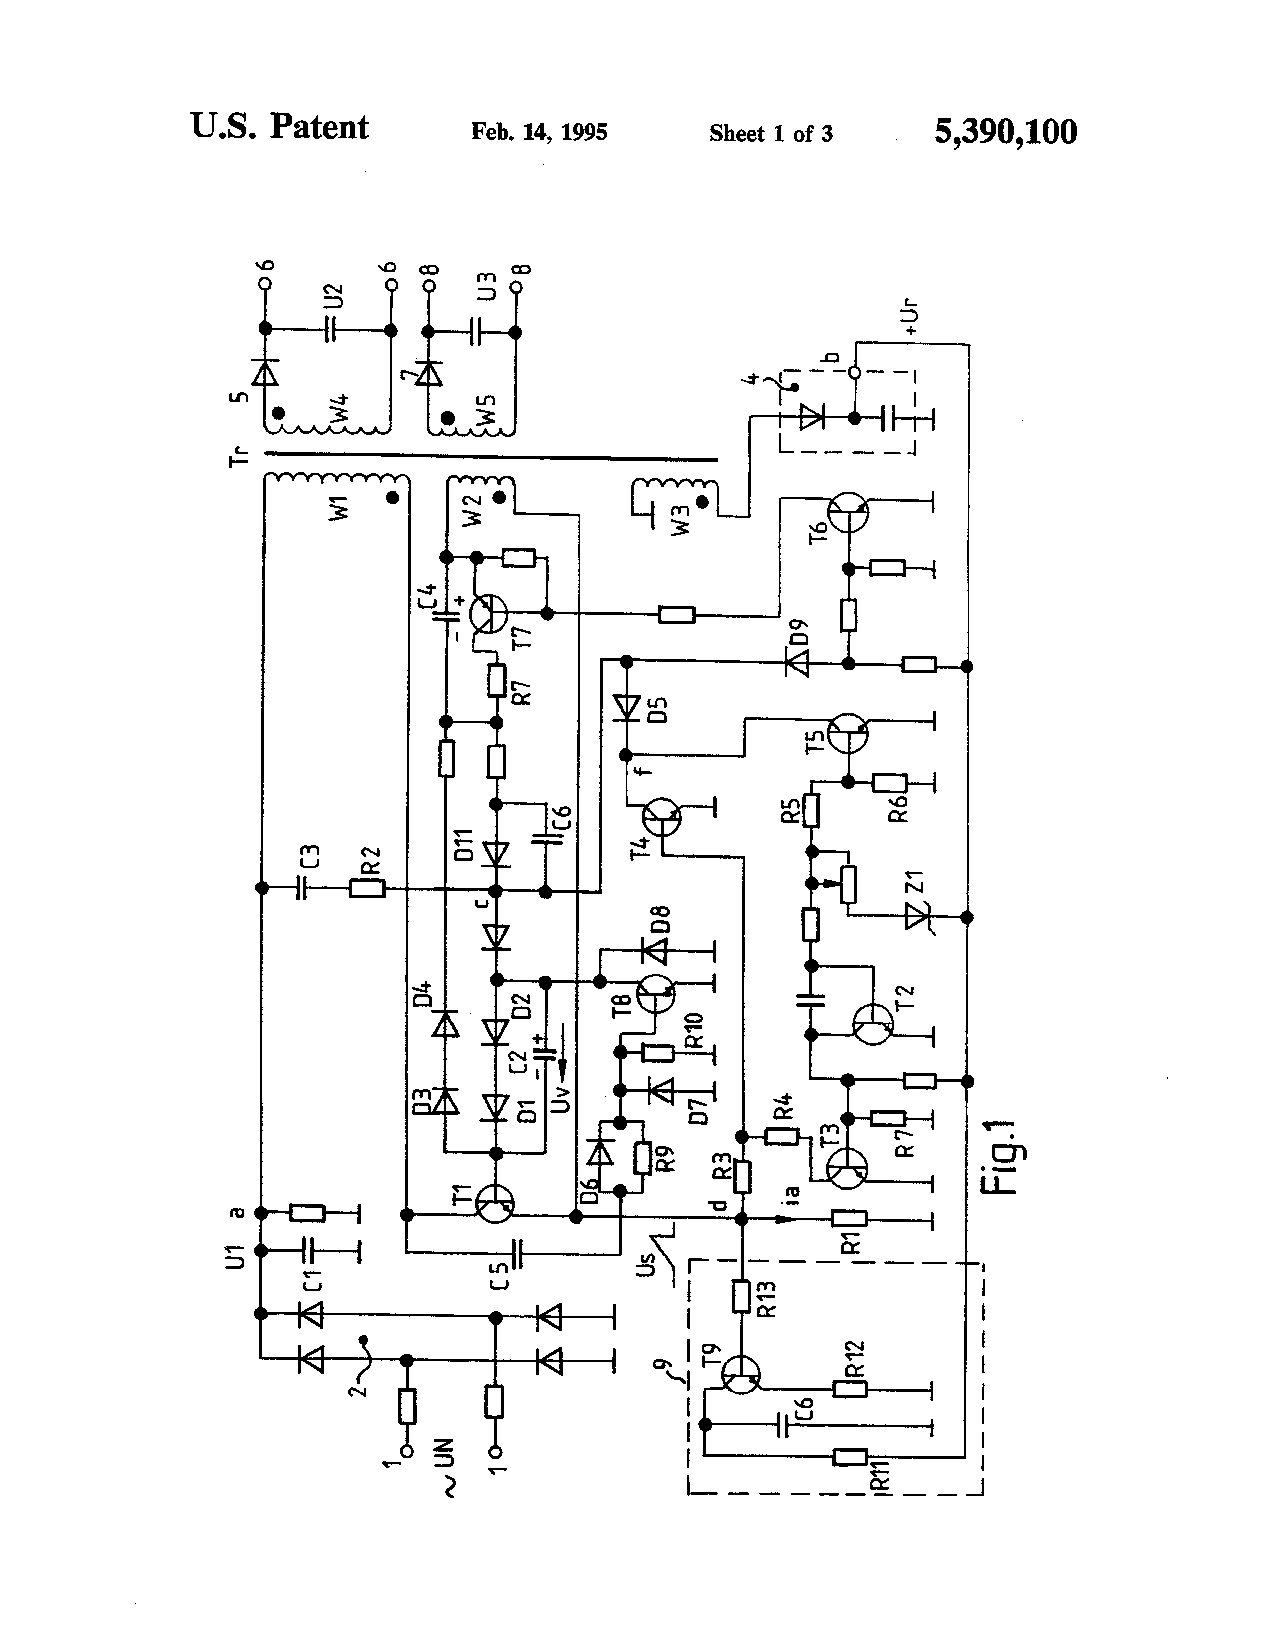
\includegraphics[width=0.7\textwidth]{graphics/Schema}}
	\caption{Schema}
	\label{fig:Schema}
\end{figure} 
\newpage
\subsection{Claim-Chart}\label{sec:Claim-Chart}
In dieser Claim-Chart wird ein Patentverlezugsprozess durchgeführt, nachfolgendes Gerät, welches nach Schema \ref{fig:CCHSchema} und \ref{fig:CCHSchema2} enspricht wurde analysiert.\\
\\

\begin{tabular}{|l|l|l|}
	\hline 
\textbf{US5390100 Palata Claim 1}& &    \\ 
	\hline 
 A freely oscillating switched-mode &A1 & freely oscillating\\
 power supply comprising:	& A2 &switched-mode  \\ 
	\hline 
a transformer having a primary winding,& B1 &primary winding\\
a secondary winding for providing &B2,B3 &secondary winding\\ 
an output voltage, and a regulating& B4&regulating winding\\
winding for providing a& & \\
measuring voltage; & &	 \\
	\hline 
a switching transistor, having a cutoff& C1 & switching transistor \\
voltage and being coupled to said  &C2  &coupled to said primary winding \\
primary winding for controlling & & \\
current therein;	&  &  \\ 
	\hline 
means for generating a control voltage& D1 & means for generating a control voltage\\
coupled to said measuring voltage;	&  & \\ 
	\hline 
first feedback means for varying said & E1 &first feedback\\
cutoff voltage responsive to said  &  &\\
control voltage when said control & &\\
voltage exceeds a first threshold value;  & &\\ 
	\hline 
second feedback means responsive to& F1&secound feedback\\
said control voltage for initiating  &  &\\
burst mode operation of said switching& & \\
transistor when said control voltage & &\\
exceeds a second threshold value.	&  &  \\ 
	\hline 

\end{tabular} 

\begin{figure}[h!]
	\centering
	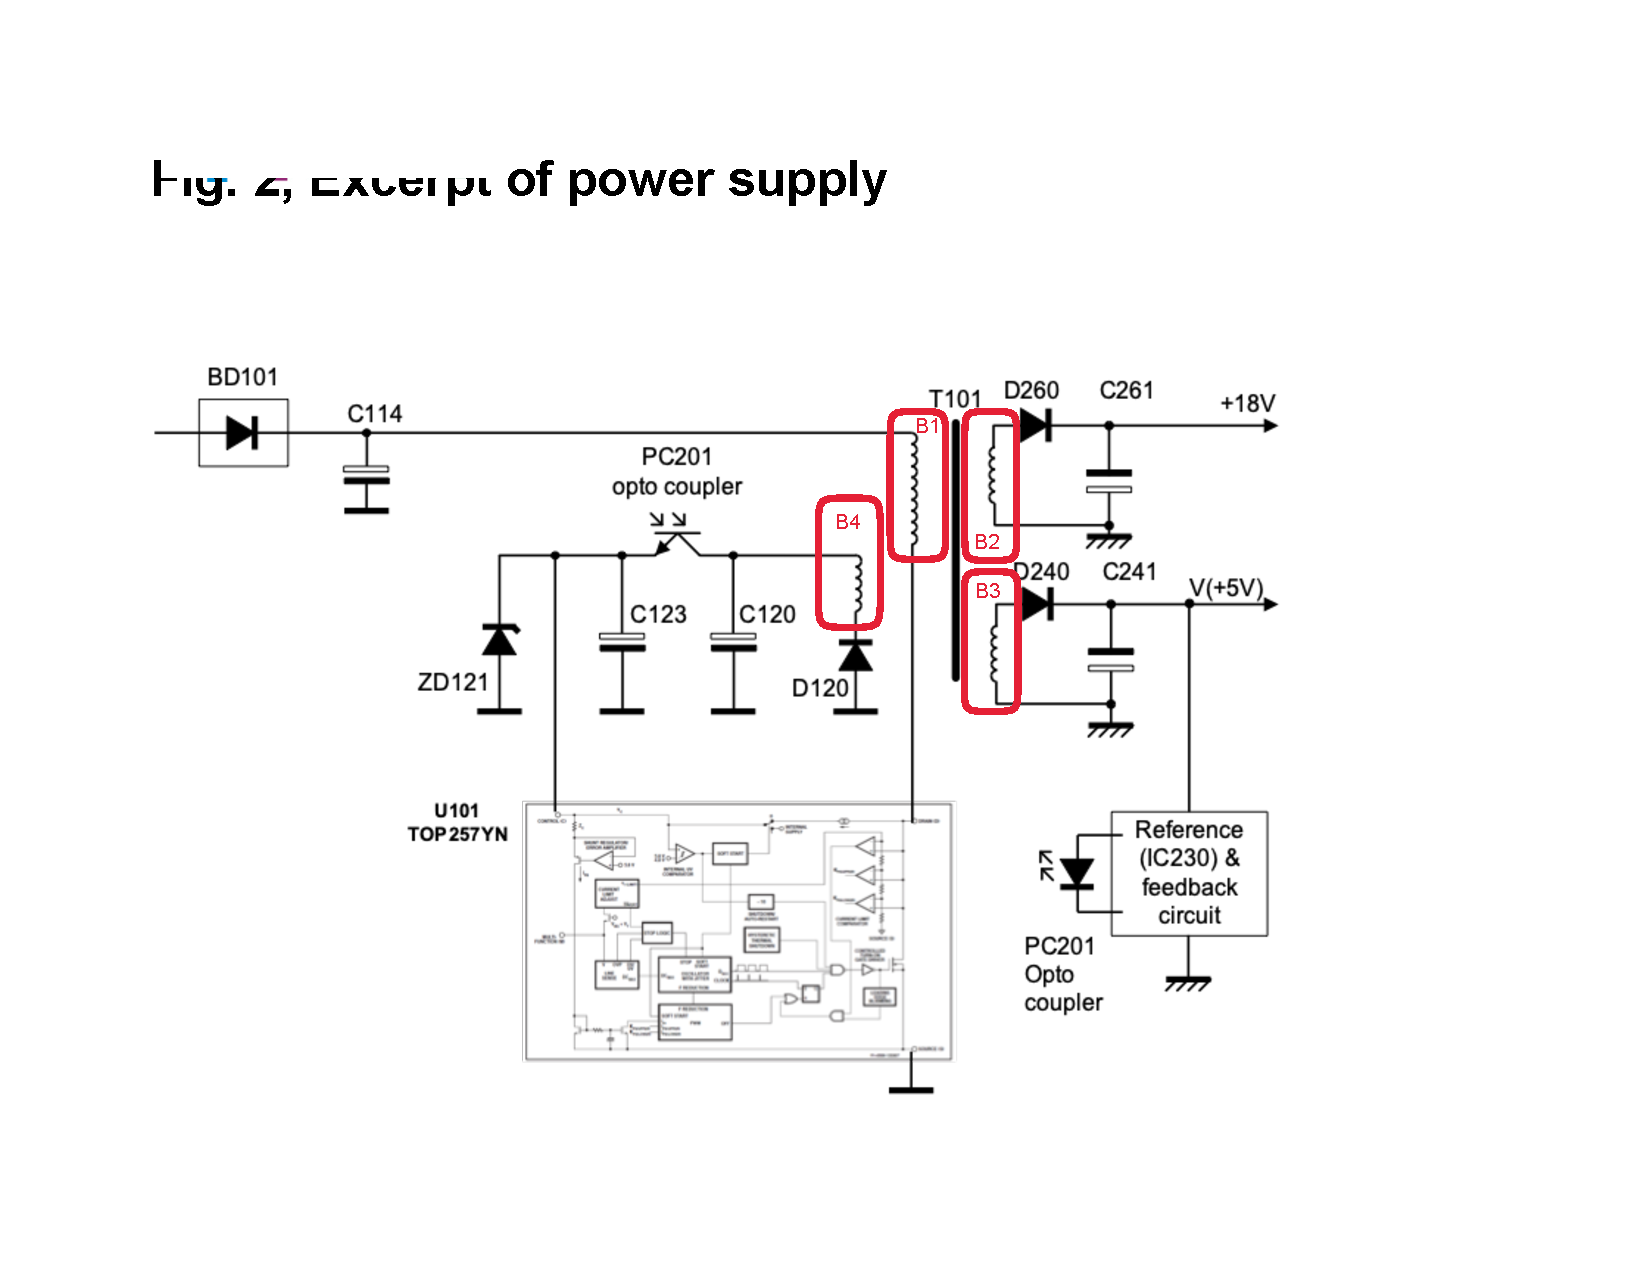
\includegraphics[trim = 20mm 20mm 50mm 50mm, clip, width=1\textwidth]{graphics/SchemaClaim}
	\caption{Claim Chart Schema Schaltnetzteil}
	\label{fig:CCHSchema}
\end{figure} 
\newpage

\begin{figure}[h!]
	\centering
	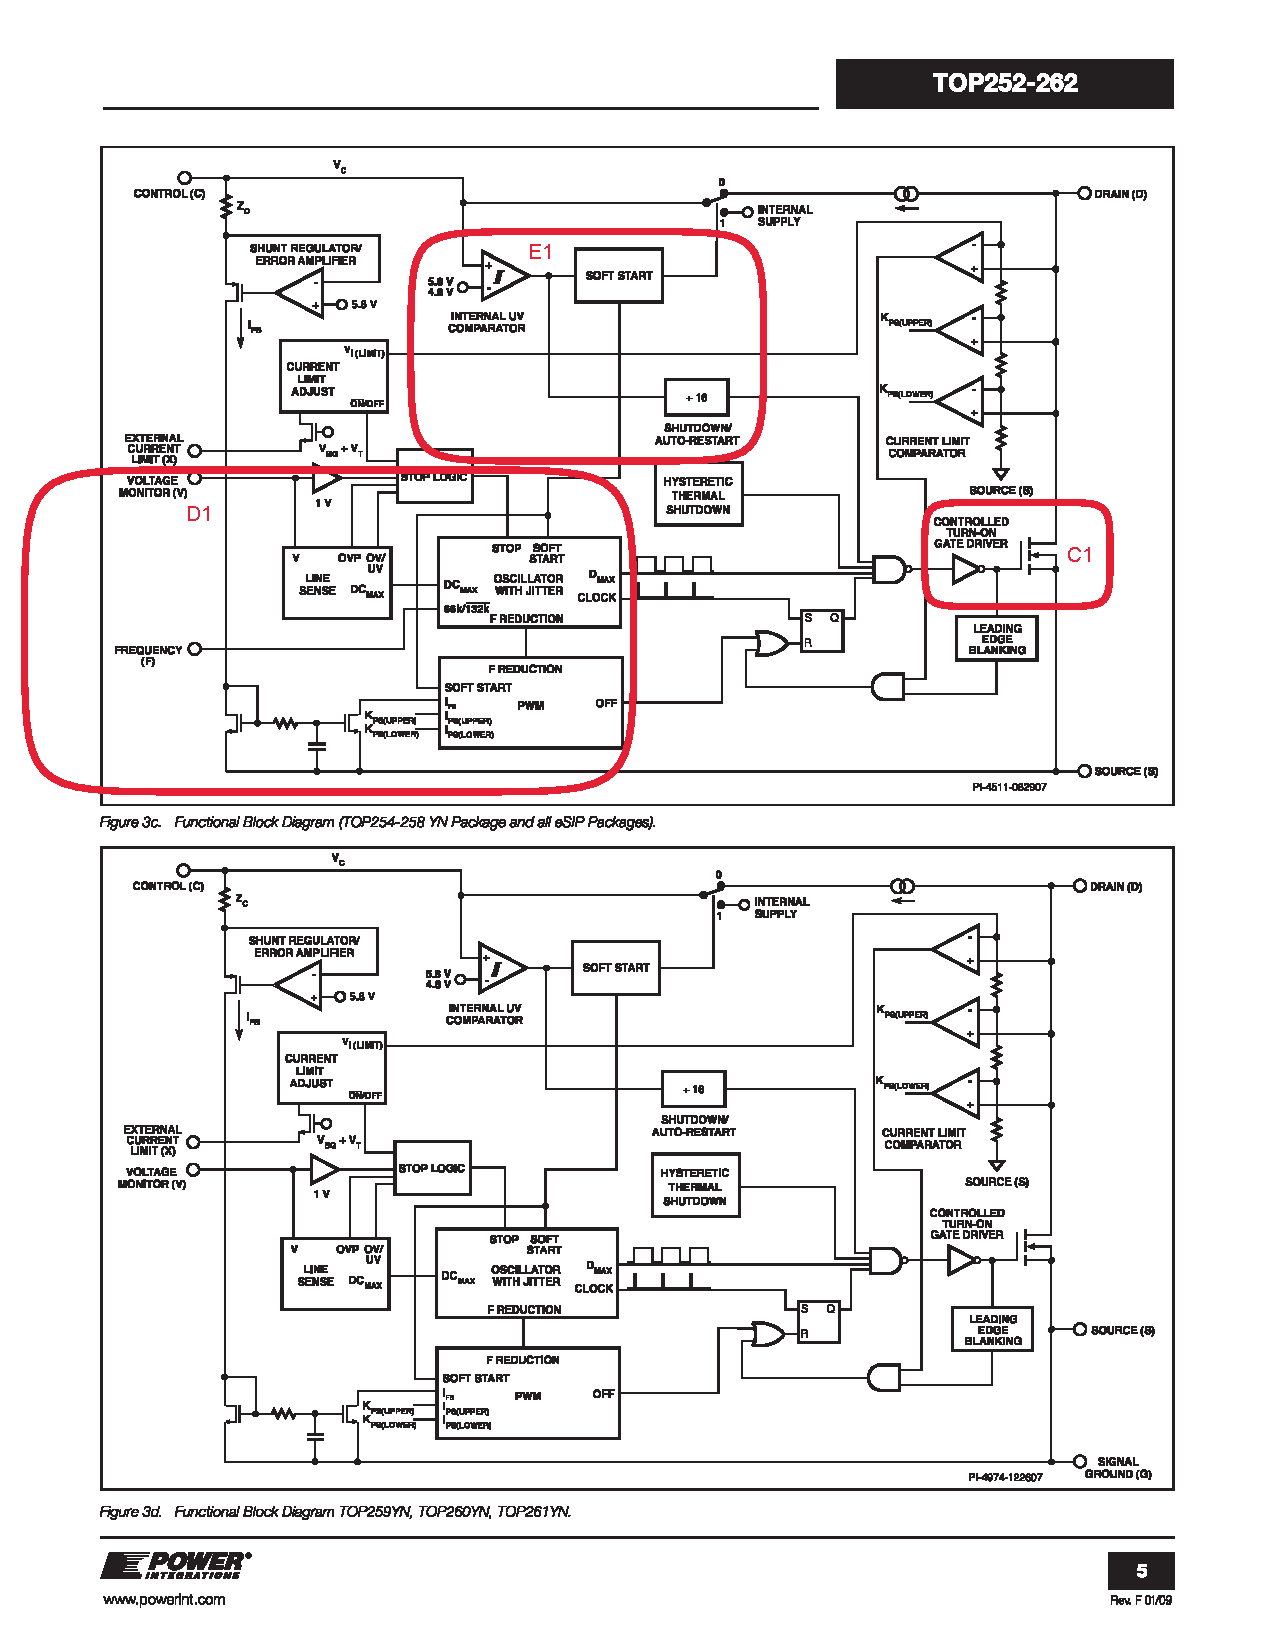
\includegraphics[trim = 1mm 142mm 1mm 20mm, clip, width=1\textwidth]{graphics/SchemaClaim2}
	\caption{Claim Chart Schema TOP257YN}
	\label{fig:CCHSchema2}
\end{figure} 